% !TeX spellcheck = de_DE

\setchapterpreamble[u]{%
\renewcommand{\dictumwidth}{0.8\linewidth}
\dictum[Bundesministerium für Digitales und Verkehr\footnote{\url{https://www.dipul.de/homepage/de/informationen/allgemeines/was-ist-eine-drohne}}]{Ein UAS besteht aus einem unbemannten Luftfahrzeug und dessen Ausrüstung. Die Steuerung kann entweder von einem Menschen oder von einem integrierten oder ausgelagerten Computer durchgeführt werden. Dadurch kann eine Drohne auch ein teil- oder vollautonomes Luftfahrzeug darstellen.}
}
\chapter{Grundlagen im Themenbereich autonomer Drohnenflug}

Der englische Fachbegriff für Drohnen lautet \enquote{\gls{uas}}. Er stammt vorrangig aus dem militärischen Bereich und beschreibt den Flugkörper selbst und etwaige Zusatzgeräte (Waffen). Heutzutage wird vermehrt der Begriff \enquote{\gls{uav}} verwendet, so auch fortwährend in dieser Arbeit. Aus dem Modellbau sind \gls{uav} in Form von fernsteuerbaren Flugzeugen, Helikoptern und Multicoptern bekannt. Drohne wird häufig als Synonym für letztere genutzt. Eine häufige Anwendung spielt dabei der autonome Flug, bei dem Anweisungen vom Bediener kommen, die automatisiert durchgeführt werden. So kann eine Drohne auch zu gewerblichem Einsatz kommen, bspw. in den folgenden Bereichen: Landwirtschaft, Wettervorhersage, Vermessung, Bevölkerungsschutz und Transport.

Zur Einstufung des automatisierten Verhaltens von Drohnen definiert die European Cockpit Association AISBL 6 \enquote{Level} (Klassen), veranschaulicht in Grafik \ref{fig:automation_levels}.
Verfügbare \gls{uav} implementieren bereits automatische Funktionen der unteren Level, wie bspw. Regelung zur Flugstabilität und dem Halten einer Flugrichtung. Interessant sind die oberen Level, beginnend bei Level 3:

\begin{compactenum}[{Level} 1]
    \setcounter{enumi}{2}
	\item - Bedingte Automation: Das \gls{uav} kann bestimmte Teilaufgaben in definierter Umgebung selbsttätig durchführen. Ein Pilot muss immer anwesend sein, um im Störungsfall einzugreifen.
	\item - Hohe Automation: Die gesamte Flugsteuerung und Ausfallsicherung wird eigenständig durchgeführt. Kein Pilot wird benötigt, jedoch muss das Verhalten des \gls{uav} überwacht werden.
	\item - Vollständige Automation (Autonomie): Eigenständige Flugplanung von Start über Flugstrecke bis Landung. Mit derzeitigen Mitteln nicht realisierbar\footnote{siehe https://twitter.com/elonmusk/status/1411280212470366213}.
\end{compactenum}

\begin{figure}[!h]
	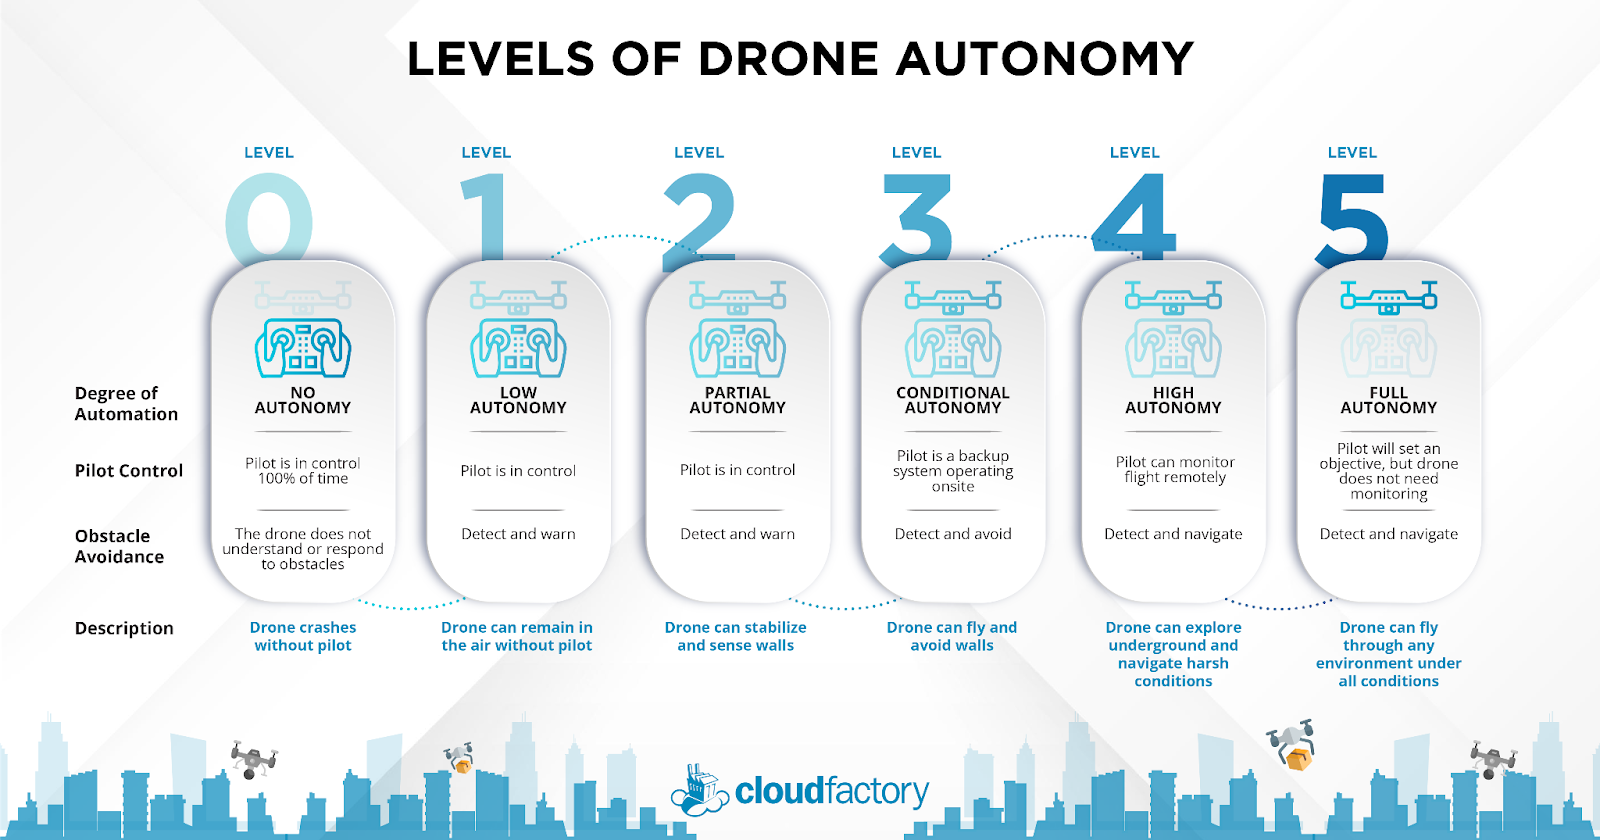
\includegraphics[width=0.7\linewidth]{images/drone_autonomy_levels.png}
	\caption[Einteilung Automationsklassen von \gls{uav}]{Einteilung Automationsklassen von \gls{uav}: Vom niedrigsten Level (0) zum höchsten Level (5) steigt der Automationsgrad, von \cite{cloudfactoryBreakingLevelsDrone}).}
	\label{fig:automation_levels}
	\end{figure}

Das \gls{lba} erlässt zudem Regelungen, wonach ein autonomer Flug \enquote*{[...] derzeit nicht zulässig [ist]; Fernpiloten müssen jederzeit eingreifen können. [...]}\cite{openuavadminDatenverbindungUndFlugmodi}.  

Der bisherige Stand des Projektes steht im Übergang von Automationsklasse 3 auf Klasse 4. Allerdings fehlen generalisierte Anwendungsfälle (später gezeigt) sodass die Drohne noch nicht wie gewünscht, Hindernissen ausweicht (das bisherige Verhalten beschränkt sich auf sicheres Landen beim Erkennen von Hindernissen).

%
%\begin{figure}[!h]
%	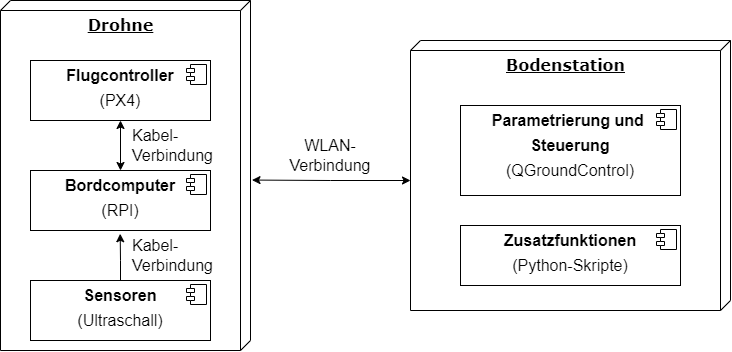
\includegraphics[width=\linewidth]{images/setup_initial_simple.drawio.png}
%	\caption{Gesamtbild Zusammenwirken der Bauteile der Drohne}
%	\label{fig:setup_initial}
%	\end{figure}
%
%
%Die Verwendung von \gls{ros} \cite[Kapitel 3.6.1]{wirthErweiterungBestehendenDrohne2022} als treibende Software zur Automatisierung ist bisher weder ausreichend entwickelt noch empfohlen \cite{haraldwirthNachfolgerInfoStudienarbeitAutonome2022}, aber doch notwendig für eine erfolgreiche Umsetzung des Projektes \cite[Kapitel 9.1]{wirthErweiterungBestehendenDrohne2022a}.
%Außerdem soll zur Automatisierung auf dem \gls{rpi} das Framework \gls{ros} verwendet werden, wie in \cref{chap:ros} zum Einsatz.

Wie in \cref{chap:sota} erläutert, wird die Modelldrohne Holybro S500 verwendet. Um diese Fliegen zu dürfen, bestehen in Deutschland mehrere Vorraussetzungen\footnote{\url{https://lba-openuav.de/onlinekurs/lehrmaterial}}:
\begin{compactitem}
	\item Drohnenführerschein: Unterkategorie A2 (\gls{uas} bis $4kg$, $5m$ Abstand zu Menschen, kein Überfliegen von Menschenansammlungen, nur auf Sichtweite fliegen)
	\item Höhenmesser: die maximale Flughöhe von $120m$ darf nicht überschritten werden
	\item Fernidentifizierung: Pflicht zum Mitführen eines ADS-B Transmitters\footnote{\url{https://de.wikipedia.org/wiki/Automatic_Dependent_Surveillance}} 
	\item Haftpflichtversicherung: Pflicht zum Versichern und Kennzeichnen der Drohne
	\item \enquote{Filmen, fotografieren oder das Anfertigen von Tonaufnahmen ist verboten, wenn: [...] die Aufnahmen für Gesichtserkennung oder andere automatisierte Prozesse verwendet werden}
\end{compactitem}

Somit der Einsatz der Drohne im öffentlichen Raum streng untersagt. Tests beschränken sich auf Flüge nahe am Boden, fernab der Zivilisation.

\section{Peripherie an der Drohne}
Im Flugcontroller integriert sind mehrere Sensoren (Beschleunigung, Gyroskop, Magnetometer, Barometer). Neben diesen besitzt das Modell einen dedizierten \gls{gps}-Empfänger. Nachfolgend ist dargestellt, wie diese Sensoren ausgewertet werden können.

%\subsection{Kommunikation mit dem Flugcontroller}\label{chap:drone_coms} Der Flugcontroller kann als eigenständige Einheit betrieben werden. Dabei kann die Drohne mittels Fernsteuerung gesteuert werden. In diesem manuellen Betrieb ist die Drohne nicht programmierbar.\newline Für zusätliche Funktionen stellt der Flugcontroller einen USB-Port und mehrere Telemetry-Ports bereit. Alle Daten zu und vom Flugcontroller werden mit dem \gls{mav}\footnote{\url{https://mavlink.io/en/}}-Protokoll übertragen. Die Daten können von Bodenstation oder entsprechenden Anwendungen ausgewertet werden. Mit der USB-Verbindung kann eine direkte Verbindung zu einem PC hergestellt werden. Somit lässt sich die Drohne einrichten, allerdings muss die Kabelverbindung zum Flug getrennt werden. Auch wird zur allgemeinen Flugsteuerung davon abgeraten die USB-Schnittstelle zu verwenden, da es bei der Datenübertragung zu Verzögerungen kommen kann.\newline Der auf die Drohne montierte \gls{rpi} kommuniziert mit dem Flugcontroller über den Telemetry-Port. Hierbei wird eine UART-Verbindung (bidirektionale Kommunikation über je eine Signalleitung) verwendet, da diese im Gegensatz zu USB einfacher zu programmieren ist und verzögerungsfrei arbeitet.\newline Das \gls{mav}-Protokoll zeichnet sich durch eine allgemein hohe Effizienz (geringer Overhead) aus. Nachrichten werden nach Themengebieten (z.B. Nachrichten vom Typ \textit{HIGHRES\_IMU} liefern Sensordaten) geordnet. Somit lässt sich eine bestimmte Eigenschaft von Interesse auslesen bzw. einspeisen. Um verlässliche Resultate beim Übertragen der Daten zu erhalten, enthalten so gut wie alle Nachrichten den Zeitpunkt des Absendens.\newline Der Flugcontroller kann konfiguriert werden nur Nachrichten bestimmter Typen zu versenden, um die Rechenlast zu verringern und höhere Übertragungsraten zu erlauben. Zu den möglichen Einstellungen zählen bspw. \textit{Normal} (Verbindung zu Bodenstation) oder \textit{Onboard} (Verbinfung zu mitgeführtem Computer) wobei ca. 40 respektive 50 Nachrichtentypen versendet werden. Wird die Einstellung \textit{Normal} verwendet, so werden keine Nachrichten vom Typ \textit{HIGHRES\_IMU} versendet. Außerdem wird für jeden Nachrichtentyp die Frequenz festgelegt, sie beträgt bspw. für die \textit{HIGHRES\_IMU} $50Hz$. 

%\subsection{Sensoren des Flugcontrollers} Ausgelesen vom Flugcontroller werden die Sensoren der \textit{HIGHRES\_IMU}. Dabei werden Messpunkte mit hoher Frequenz und Auflösung bereitgestellt. Eine Verarbeitung muss die Daten filtern um weitere Berechnungen durchführen zu können. Zur Verwendung kommt \gls{ros}, 

\subsection{Navigation mittels GPS}
Die Navigation der Drohne erfolgt vorrangig über \gls{gps}. Mit solchem System können die aktuelle Position und Geschwindigkeit festgestellt werden. Für ein reales System muss ein eventueller Ausfall der \gls{gps}-basiertern Navigation in Betracht gezogen werden, denn \gls{gps} setzt klare Sicht zum Himmel und eine Verbindung zu mindestens 4 Satelliten voraus. [Quelle]

Fällt das \gls{gps} aus, ist die Drohne jedoch noch nicht völlig blind. Beschleunigungssensor, Gyroskope und Kompass bilden eine \gls{imu}, mit deren Daten mittels eines \textit{Extended Kalman Filter} die ungefähre Position berechnet werden kann. Das Ergebnis kann durch das Überlagern der Messwerte mehrerer Sensoren verbessert werden, bspw. indem sich an einem Kamerabild mit den bereits bekannten Abständen zu Objekten orientiert wird. 
%Der Flug der Drohne kann trotzdem zu jeder Zeit von Umwelteinflüssen (bspw. Wind) beeinflusst werden. Dabei kann sich die Position trotzdem unbemerkt verändern.

Ein weiteres Problem ist die totale Abhängigkeit von \gls{gps} in Bezug auf Zielfindung. Selbst wenn die Drohne direkt über dem Zielpunkt fliegt, aber \gls{gps} ausfällt, kann sie keine Erfolg verzeichnen. Für die Flugplanung wäre folglich ein zweiter Sensor von notwendig, der ohne \gls{gps} zum Zielpunkt navigieren kann. Für das Aufwinden des Zieles stehen mehrere Technologien zur Verfügung:
\begin{compactdesc}
    \item[Ortung] eines Sender (Ultraschall oder Infrarot) welcher durchgängig Signale sendet. Die Drohne bewegt sich dann immer auf den Sender zu.
    \item[Erkennung] einer Struktur oder Bildes (Marker) mittels Kamera.
\end{compactdesc}
%
%\subsection{Routenplanung}
%Weiterhin kann mit \gls{gps} und dem vorher eingeführten Magneten-Prinzip (siehe \cref{chap:sota}) kein Erfolg bei der Navigation erzielt werden, falls das Ziel nicht auf direktem Weg erreichbar ist. [noch ein Bild] Die Konsequenz ist, dass ein autonomer Flug eine Umgebungskarte und Routenplanung benötigt.
%Dazu muss die Drohne muss ihre Umgebung per Sensor wahrnehmen und ein 3D-Modell der Umgebung erstellen. Dazu werden weitere Sensoren und ein Wegfindungs-Algorithmus benötigt.
%
%Eine verfügbare Routenplanung soll den optimalen Weg von einem gegeben Start zum Ziel finden.
%Für die Drohne, die sich auf beliebigem Weg durch die Luft bewegen kann, ist die Luftlinie eine erste und sehr gute Näherung hierfür.
%Um den optimalen Weg zu finden, muss der Ansatz verschiedene Faktoren auf dem Weg berücksichtigen. Es ergeben sich wirksame Beispiele:
%\begin{compactdesc}
%	\item[Hindernisse:] Ein Berg mit Tunnel versperrt den Weg. Sollte die Drohne den Tunnel bemerkt haben, sollte sie hinein fliegen oder um den Berg herum?
%	\item[Luftwiderstand:] Gegenwind bremst die Drohne stark ab. Sollte sich die Drohne näher am Boden/ weiter in der Luft aufhalten, um dem Wind zu entgehen? 
%\end{compactdesc}
%Das Beispiel des Luftwiderstands erscheint komplex und erfordert spezielle Sensoren zur Messung. Deshalb kann es in dieser Arbeit nicht näher betrachtet werden.
%Eine gezielte Umgehung von Hindernissen sollte allerdings Teil des autonomen Fluges sein.
%

\subsection{Hinderniserkennung durch Ultraschallsensoren}\label{chap:ultrasonic}
Mit einem Ultraschallsensor kann der Abstand zu Objekten gemessen werden. 

Das Prinzip der Ultraschallortung besteht aus 3 Schritten:
\begin{compactenum}
	\item Aussenden des Messimpulses. Daraufhin generiert der Sensor Ultraschall-Impulse.
	\item Empfangen der Messimpulse. Der Sensor setzt ein Signal wenn ein Echo empfangen wird.
	\item Auswerten der Signallaufzeit. Die Impulse bewegen sich mit Schallgeschwindigkeit im Medium zum Messobjekt und zurück.
\end{compactenum}

Verwendet werden Ultraschallsensoren an der Drohne, welche Messimpulse in die Umgebung aussenden. Für eine exakte Auswertung der Signallaufzeit müssten Umgebungstemperatur, Luftdruck und Luftfeuchte bekannt sein. Den größten Einfluss spielt dabei die Temperatur. Druck und Feuchte wirken nur mit jeweils maximal auf das Ergebnis ein 5\% bzw. 2\%.\newline
Die Formel zur Bestimmtung der Entfernung eines Objektes lautet ist gegeben in Formel \ref{mat:dist_by_t}. Benötigt wird die Schallgeschwindigkeit $c_{20}$ bei $20$\textcelsius und der Temperaturkoeffizient $\alpha_{20}$\cite[Seite 152]{grudenSensorikUndMesswertverarbeitung2022}.
\begin{align}
	s &=\frac{1}{2}c\cdot t\\
	&=\frac{1}{2}c_{20}(1+\alpha_{20}(\vartheta-20\textrm{\textcelsius})) t	\label{mat:dist_by_t}
\end{align}

\section{Bilderkennung und Obstacle Avoidance}
Mannigfaltige Prinzipien fallen in den Bereich der Bilderkennung. Der Fokus dieses Projektes, das Erkennen und Ausweichen von Hindernissen wird \enquote{Obstacle Avoidance} genannt. Es ist nicht zu verwechseln mit \enquote{Obstacle Detection}, dem Erkennen und Klassifizieren von Bildinhalten. Nachfolgend vorgestellt werden Techniken die hier zum Einsatz kommen könnten. 
\paragraph*{SLAM Algorithmus}\label{chap:slam}
\Gls{slam} Techniken entstanden bereits in den 1980-1990 Jahren und wird bspw. bei Robotern eingesetzt, die in Hallen navigieren (kein \gls{gps} verfügbar). Dazu kommen mit Kamerasysteme in Verbindung mit Entfernungssensor (Sonar, Radar, Lidar) zur Verwendung . Die Ergebnisse von \gls{slam} können nicht garantiert werden und sind nicht reproduzierbar, weshalb es in keinen kritischen Umgebungen (bspw. wenn Verletzungsrisiko besteht) eingesetzt werden kann.

Allgemein wird \gls{slam} durch einen modularen Prozess beschrieben: \begin{compactdesc}
    \item[Lokalisierung:] per Motorfortschritt, \gls{imu}, Kamera, etc.\newline
    Bei v\gls{slam} kommen folgende Prinzipien zum Einsatz:
\end{compactdesc}
\begin{compactitem}
    \item Markov-Lokalisierung: Wahrscheinlichkeit des Aufenthaltsortes wird angenommen und über Zeit verfeinert. Iterativ, Ressourcenaufwendig.
	\item Kalman-Filter: Ermöglicht basierend auf Sensordaten schnelles wiederfinden aktueller Position. Anfällig bei Verlust von Kamerabildern
	\item Monte-Carlo-Lokalisierung: auch Partikelfilter genannt, nimmt Wahrscheinlichkeiten für jeden Ort an. Genauer als Markov, lineare Komplexität. Weniger Speicher als Kalman. Nachteil: Stillstand ohne sich ändernde Sensordaten
\end{compactitem}
\begin{compactdesc}
    \item[Messung:] per Reichweite, Marker in Umgebung
\end{compactdesc}
%was sollte hier noch hin

\paragraph*{Visual SLAM} 
Eine Sonderform des \gls{slam} ist Visual \gls{slam} (vSLAM). Bei diesem werden ausschließlich Kameras zur Erkennung der Umgebung eingesetzt. Der Algorithmus verwendet zusätzliche Sensordaten um die Bewegung der Kamera in die Berechnung der Position einzubeziehen.

\paragraph*{Stereokamera}\label{chap:stereovision}
Verwendet mehrere Kameras aus parallelverschobenen Bildern Tiefeninformationen zu gewinnen. also Abstand zu Punkten im Bild zu erkennen.
\paragraph*{Optical Flow}
Auswertung der Bewegung von Objekten in Videoabläufen. Kann schlecht zwischen Bewegung der Kamera und Bewegung der Objekte unterscheiden. Ungenau, da Kameras immer eine Verzerrung besitzen. 

\section{Robot Operating System}
koennte auch mal noch... ist erklaert in \cite[Kapitel 2.2]{wirthErweiterungBestehendenDrohne2022a}